%%%%%%%%%%%%%%%%%%%%%%%%%%%%%%%%%%%%%%%%%
% a0poster Portrait Poster
% LaTeX Template
% Version 1.0 (22/06/13)
%
% The a0poster class was created by:
% Gerlinde Kettl and Matthias Weiser (tex@kettl.de)
% 
% This template has been downloaded from:
% http://www.LaTeXTemplates.com
%
% License:
% CC BY-NC-SA 3.0 (http://creativecommons.org/licenses/by-nc-sa/3.0/)
%
%%%%%%%%%%%%%%%%%%%%%%%%%%%%%%%%%%%%%%%%%

%----------------------------------------------------------------------------------------
%	PACKAGES AND OTHER DOCUMENT CONFIGURATIONS
%----------------------------------------------------------------------------------------

\documentclass[a0,portrait]{a0poster}

\usepackage[portuguese]{babel}%Formata as entradas para PT-BR
%\usepackage[utf8]{inputenc}
%\usepackage{verbatim}
\usepackage[document]{ragged2e}
\usepackage{multicol} % This is so we can have multiple columns of text side-by-side
\columnsep=100pt % This is the amount of white space between the columns in the poster
\columnseprule=3pt % This is the thickness of the black line between the columns in the poster

\usepackage[svgnames]{xcolor} % Specify colors by their 'svgnames', for a full list of all colors available see here: http://www.latextemplates.com/svgnames-colors

\usepackage{times} % Use the times font
%\usepackage{palatino} % Uncomment to use the Palatino font
%\usepackage{varioref}
%\usepackage{hyperref}
%\usepackage{epsfig}
\usepackage{graphicx} % Required for including images
\graphicspath{{figures/}} % Location of the graphics files
\usepackage{booktabs} % Top and bottom rules for table
\usepackage[font=small,labelfont=bf]{caption} % Required for specifying captions to tables and figures
\usepackage{amsfonts, amsmath, amsthm, amssymb} % For math fonts, symbols and environments
\usepackage{mathrsfs}
\usepackage{wrapfig} % Allows wrapping text around tables and figures
\usepackage{setspace}

\begin{document}
\onehalfspacing
%----------------------------------------------------------------------------------------
%	POSTER HEADER 
%----------------------------------------------------------------------------------------

% The header is divided into two boxes:
% The first is 75% wide and houses the title, subtitle, names, university/organization and contact information
% The second is 25% wide and houses a logo for your university/organization or a photo of you
% The widths of these boxes can be easily edited to accommodate your content as you see fit

\begin{center}
\vspace*{-3.8cm}
    
\includegraphics[width=0.18\textwidth]{logo} 
	\hspace{55.5cm}
	
\includegraphics[width=0.06\textwidth]{ufms} 
	%\hspace{3.5cm}
	%
\includegraphics[width=0.1\textwidth]{cnpq}
\vspace{1,5cm}
\end{center}

\begin{minipage}[b]{1.0\linewidth} %default 0.75
\begin{center}
\Huge \textbf{T\'ITULO}\\
%\Huge \textbf{T\'ITULO (EM MAI\'UšSCULO)}\\% Title
%\Huge\textit{An Exploration of Complexity}\\[2cm] % Subtitle
\huge \textbf{NOME COMPLETO DO AUTOR(A)$^{1}$, AUTOR(A)$^{2}$, AUTOR(A)$^{3}$, AUTOR(A)$^{4}$}\\
%\huge \textbf{}\\
[0.5cm] % Author(s)
\huge Nome da Universidade, UF, Brasil\\[0.4cm] % University/organization
\Large \texttt{email$^{1}$, email$^{2}$, email$^{3}$, email$^{4}$}\\
\end{center}
\end{minipage}
%
\vspace{1cm} % A bit of extra whitespace between the header and poster content


%----------------------------------------------------------------------------------------

\begin{multicols}{2} % This is how many columns your poster will be broken into, a portrait poster is generally split into 2 columns

\justify % Justify all text

%----------------------------------------------------------------------------------------
%	ABSTRACT
%----------------------------------------------------------------------------------------

%\color{Navy} % Navy color for the abstract

%\begin{abstract}
\section*{Resumo}
\vspace{-1cm}
O RESUMO deve ser claro, sucinto e explicar o(s) objetivo(s) pretendido(s), procurando justificar sua import\^ancia, os principais procedimentos adotados, os resultados mais expressivos e conclus\~oes. Se recomenda que o RESUMO n\~ao contenha f\'ormulas, cita\c c\~oes e/ou refer\^encias bibliogr\'aficas.

\vspace{1cm}

\hspace{-0,5cm}\textbf{Palavras-Chave:} m\'aximo de cinco, separadas por ponto e v\'i­rgula (;), procurando n\~ao repetir palavras do t\'i­tulo, escritas em letras min\'usculas, organizadas em ordem alfab\'etica crescente. 
%\end{abstract}

%----------------------------------------------------------------------------------------
%	Introdu\c c\~ao
%----------------------------------------------------------------------------------------

%\begin{abstract}
\section*{Introdu\c c\~ao}
\vspace{-1cm}
A introdu\c c\~ao tem como objetivo posicionar o leitor dentro do tema que est\'a sendo desenvolvido. Deve conter a delimita\c c\~ao do universo da pesquisa, problema, objetivos, justificativa, hip\'oteses, metodologia de trabalho e sua relev\^ancia. Evitar o uso de palavras e ideias repetidas. Seja objetivo e preciso em suas considera\c c\~oes, evitando que a introdu\c c\~ao do trabalho fique longa e cansativa. 
%\end{abstract}

%----------------------------------------------------------------------------------------
%	OBJETIVOS
%----------------------------------------------------------------------------------------

%\color{Navy} % Navy color for the abstract

%\begin{Objetivos}
\section*{Objetivos}
\vspace{-1cm}
O objetivo geral deve resumir e apresentar a ideia central de um trabalho, descrevendo tamb\'em sua finalidade. Os objetivos espec\'i­ficos ir\~ao dar uma maior delimita\c c\~ao ao tema, al\'em de detalhar os processos necess\'arios para a realiza\c c\~ao do trabalho.

%\end{Objetivos}

%----------------------------------------------------------------------------------------
%	Fundamenta\c c\~ao Te\'orica
%----------------------------------------------------------------------------------------

%\color{Navy} % Navy color for the abstract

%\begin{Fundamenta\c c\~ao Te\'orica}
\section*{Fundamenta\c c\~ao Te\'orica}
\vspace{-1cm}
Apresenta as refer\^encias nas quais se baseia a pesquisa:\\
\begin{itemize}
\item livros, artigos em revistas/peri\'odicos, teses de doutorado, disserta\c c\~oes de mestrado
\end{itemize}
O referencial te\'orico tem tamb\'em outras fun\c c\~oes:
\begin{itemize}
\item permite que o autor tenha maior clareza,
\item facilita a formula\c c\~ao de hip\'oteses e de suposi\c c\~oes,
\item sinaliza para o m\'etodo mais adequado \`a  solu\c c\~ao do problema,
\item permite identificar qual o procedimento mais pertinente para a coleta e o tratamento dos dados, bem como o conte\'udo do procedimento escolhido.
\item uma revis\~ao de literatura serve para verificar o que j\'a foi pesquisado do assunto. 

\end{itemize}

%\end{Fundamenta\c c\~ao Te\'orica}
%----------------------------------------------------------------------------------------
%	PROBLEM FORMULATION
%----------------------------------------------------------------------------------------

%\color{SaddleBrown} % SaddleBrown color for the introduction

%\begin{center}
\section*{Desenvolvimento e Metodologia ou Materiais e M\'etodos}
%\end{center}
%\begin{justify}
%\setlength{\parindent}{5ex} \indent \par
\vspace{-1cm}
Descrever adequadamente o desenvolvimento e a metodologia utilizada para desenvolver o trabalho. Deve ser pertinente ao tema, procurando alcan\c car os objetivos j\'a apresentados.\\
Caso use equa\c c\~oes, numerar descrevendo os par\^ametros.\\
 Figuras, tabelas e gr\'aficos devem ser apresentados com tamanho, qualidade e detalhes suficientes para a interpreta\c c\~ao e composi\c c\~ao gr\'afica final. 
Citar a fonbte da ilustra\c c\~ao, tabela e gr\'afico e, caso seja do pr\'oprio autor, citar como Fonte: elaborada pelo autor.
As legendas e fontes das figuras, tabelas e gr\'aficos devem ser escritos em fonte Times New Roman, tamanho 10 e o texto deve estar centralizado, em negrito e seguir o padr\~ao de numera\c c\~ao sucessivo ar\'abico. Centralizar as Figuras, Tabelas e Gr\'aficos.
\textbf{Gr\'aficos e figuras:} devem apresentar-se sem bordas; a legenda deve ser posicionada logo abaixo da figura ou gr\'afico. Usar imagens coloridas se for necess\'ario destacar alguma informa\c c\~ao da Figura ou Gr\'afico.

 
\textbf{Tabelas:} evitar tabelas extensas e dados sup\'erfluos; adequar seus tamanhos ao espa\c co \'util do papel e colocar, na medida do poss\'i­vel, apenas linhas cont\'i­nuas horizontais. As legendas devem ser autoexplicativas, localizadas abaixo da tabela, como no exemplo a seguir. 

\vspace{2cm}
\begin{minipage}[b]{1.0\linewidth}
\begin{center}
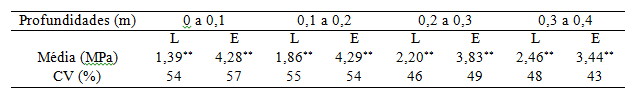
\includegraphics[width=37cm]{tabela.png}
\captionof{figure}{An\'alise do \'Indice de Cone (IC) nas linhas (L) e entrelinhas (E) de cana nas diferentes profundidades amostradas. Fonte: OLIVEIRA et al., 2008.}
\end{center}
\end{minipage}
\vspace{-1cm}
%\end{justify}


%----------------------------------------------------------------------------------------
%	NUMERICAL RESULTS 
%----------------------------------------------------------------------------------------

\section*{Resultados}
\vspace{-1cm}
Apresentar os resultados de maneira organizada e l\'ogica, fornecendo ao leitor as informa\c c\~oes mais representativas. \'E comum o uso de figuras e tabelas para ilustrar os dados apresentados de maneira a facilitar a compreens\~ao dos resultados obtidos. As legendas devem ser autoexplicativas, localizadas abaixo da tabela, como no exemplo a seguir.

\vspace{2cm}
\begin{minipage}[b]{1.0\linewidth}
\begin{center}
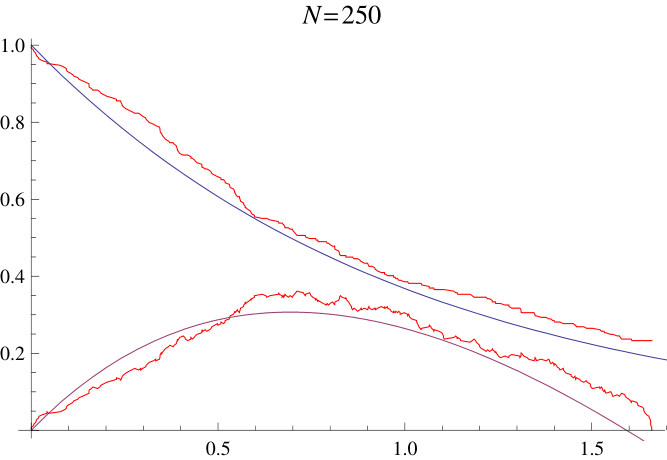
\includegraphics[scale=0.8]{figura.png}
\captionof{figure}{Descri\c{c}\~ao da figura aqui.}
\end{center}
\end{minipage}
\vspace{-1cm}
%\end{justify}


%

%\begin{wraptable}{l}{12cm} % Left or right alignment is specified in the first bracket, the width of the table %is in the second
%\begin{tabular}{l l l}
%\toprule
%\textbf{Treatments} & \textbf{Response 1} & \textbf{Response 2}\\
%\midrule
%Treatment 1 & 0.0003262 & 0.562 \\
%Treatment 2 & 0.0015681 & 0.910 \\
%Treatment 3 & 0.0009271 & 0.296 \\
%\bottomrule
%\end{tabular}
%\captionof{table}{\color{Green} Table caption}
%\end{wraptable}



%----------------------------------------------------------------------------------------
%	CONCLUSIONS
%----------------------------------------------------------------------------------------

%\color{SaddleBrown} % SaddleBrown color for the conclusions to make them stand out

\section*{Conclus\~oes}
\vspace{-1cm}
Devem basear-se, exclusivamente, nos resultados do trabalho. Ressaltar se os objetivos expostos inicialmente foram cumpridos e se a hip\'otese foi confirmada. Aspectos metodol\'ogicos tamb\'em devem ser abordados: dificuldades durante a pesquisa, resultados obtidos e qual o significado dos mesmos dentro da \'area de pesquisa. Quando poss\'i­vel, inserir outros tipos de estudos que poderiam ser feitos utilizando o mesmo tema e/ou outros aspectos a serem abordados a partir dos resultados apresentados.


%\color{DarkSlateGray} % Set the color back to DarkSlateGray for the rest of the content

%----------------------------------------------------------------------------------------
%	REFERENCIAS
%----------------------------------------------------------------------------------------
\vspace{-1cm}
\nocite{*} % Print all references regardless of whether they were cited in the poster or not
\begin{thebibliography}{100}

\bibitem{Boldrini} 
J. L. Boldrini, S. I. R. Costa, V. R. Ribeiro, and H. G. Wetzler. {\it   \'{A}lgebra Linear e Aplica\c{c}\~{o}es}, 3a. edi\c{c}\~{a}o. Harbra, S\~{a}o Paulo, 1984.

\bibitem{Cuminato}
J. A. Cuminato and V. Ruas. Unification of distance inequalities for linear variational problems, 
{\it Comp. Appl. Math.}, 2014. DOI: 10.1007/s40314-014-0163-6.

\bibitem{Diniz1}
G. L. Diniz, A mudan\c{c}a no habitat de popula\c{c}\~{o}es de peixes: de rio a represa -- o modelo matem\'{a}tico, Disserta\c{c}\~{a}o de Mestrado em Matem\'{a}tica Aplicada, Unicamp, 1994.

\bibitem{Jafelice} R. M. Jafelice, L. C. Barros and R. C. Bassanezi. Study of the dynamics of HIV under 
treatment considering fuzzy delay, {\it Comp. Appl. Math.}, 33:45--61, 2014.

\bibitem{Santos} I. L. D. Santos e G. N. Silva. Uma classe de problemas de controle \'{o}timo 
em escalas temporais, {\it Proceeding Series of the Brazilian Society of Computational and 
Applied Mathematics}, volume 1, 2013. DOI: 10.5540/03.2013.001.01.0177.
\end{thebibliography}


\section*{Agradecimentos (Opcional)}
\vspace{-1cm}
Inserir, ap\'os as conclus\~oes, de maneira sucinta os agradecimentos. Se o projeto for financiado por alguma ag\^encia de fomento, citar a fonte.



%----------------------------------------------------------------------------------------

\end{multicols}
\end{document}